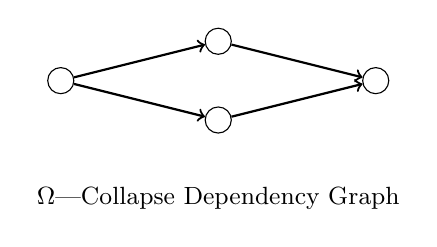
\begin{tikzpicture}[
    node/.style={circle, draw=black, fill=white, minimum size=6pt},
    arrow/.style={->, thick}
]

\node[node] (A) at (0,0) {};
\node[node] (B) at (2,0.5) {};
\node[node] (C) at (2,-0.5) {};
\node[node] (D) at (4,0) {};

\draw[arrow] (A) -- (B);
\draw[arrow] (A) -- (C);
\draw[arrow] (B) -- (D);
\draw[arrow] (C) -- (D);

\node at (2,-1.5) {\small $\Omega$---Collapse Dependency Graph};

\end{tikzpicture}